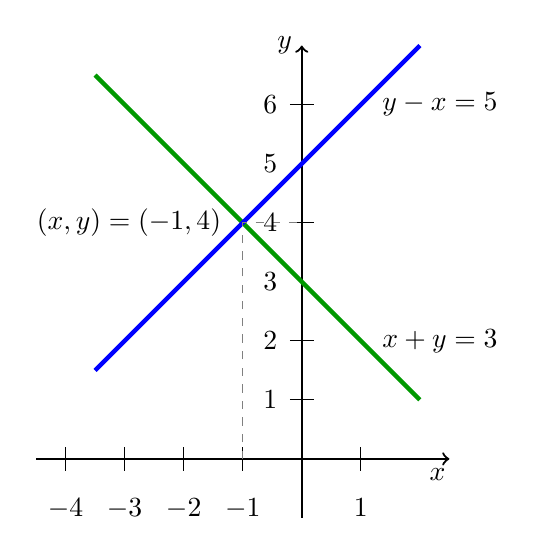
\begin{tikzpicture}[scale=0.75]
      \draw[thick, ->](-4.5,0) -- (2.5,0);
      \draw[thick, ->](0,-1) -- (0,7);
      \draw(-4,-0.2) -- (-4,0.2);
      \draw(-3,-0.2) -- (-3,0.2);
      \draw(-2,-0.2) -- (-2,0.2);
      \draw(-1,-0.2) -- (-1,0.2);
      \draw(1,-0.2) -- (1,0.2);
      \draw(-0.2,1) -- (0.2,1);
      \draw(-0.2,2) -- (0.2,2);
      \draw(-0.2,4) -- (0.2,4);
      \draw(-0.2,6) -- (0.2,6);
      \draw[green!60!black, ultra thick, domain=-3.5:2] plot (\x, {3-\x});
      \draw[blue, ultra thick, domain=-3.5:2] plot (\x, {\x+5});
      \node[right] at (1.2,2){$x+y=3$};
      \node[right] at (1.2,6){$y-x=5$};
      \draw[help lines,dashed](-1,0)--(-1,4)--(0,4);
      \node[below] at (-4,-0.5){$-4$};
      \node[below] at (-3,-0.5){$-3$};
      \node[below] at (-2,-0.5){$-2$};
      \node[below] at (-1,-0.5){$-1$};
      \node[below] at (1,-0.5){$1$};
      \node[left] at (-0.25,1){$1$};
      \node[left] at (-0.25,2){$2$};
      \node[left] at (-0.25,3){$3$};
      \node[left] at (-0.25,4){$4$};
      \node[left] at (-0.25,5){$5$};
      \node[left] at (-0.25,6){$6$};
      \node[below right] at (2,0){$x$};
      \node[left] at (0,7){$y$};
      \node[left=1ex] at (-1,4){$(x,y) = (-1,4)$};
    \end{tikzpicture}
